\renewcommand{\this}{PCA}

\chapter{Principle Component Analysis (PCA)}
\section{Matrix factorization as a tool}
The core concept of principle component analysis is 
making use of matrix factorization techniques. These 
techniques, as the name implies, decompose a matrix 
of interest $X \in \Real^{m \times n}$ into several 
matrices such that their product equals $X$. For 
example, an approximation of the data matrix $X$ 
could be given by the product of 
$A \in \Real^{m \times k}$ and $B \in \Real^{k \times n}$:
\\
\begin{figure}[h!]
	\centering	
	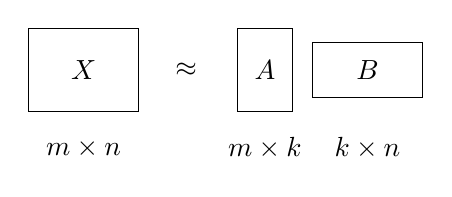
\begin{tikzpicture}
	\draw (0,0) node[shape=rectangle, 
					 draw=black, 
					 minimum width = 40, 
					 minimum height = 30](x){$X$};
	\draw node[below of = x] (times) {$m \times n$};
	\draw node[right of = x, xshift = 2ex] (apr){$\approx$};
			
	\draw node[right of = apr, 
			   shape=rectangle, 
			   draw=black, 
			   minimum width = 20, 
			   minimum height = 30](A){$A$};
			   
	\draw node[below of = A] (times) {$m \times k$};
			
	\draw node[right of = A, 
			   shape=rectangle, 
			   draw=black, 
			   minimum width = 40, 
			   minimum height = 20, 
			   xshift = 2ex](B){$B$};
	\draw node[below of = B] (times) {$k \times n$};
	\end{tikzpicture}
	\label{approx}
	\caption{Example of factorization.}
\end{figure}\\
A whole range of practical problems can be written
as a matrix factorization problems. Often we can 
gain a lot of insights based on decompositions.
\\\\
In the previous example, the matrix $X$ was a $m \times n$ matrix. 
It was decomposed into $m \times k$ and $k \times n$ matrices. 
Naturally, $A$ and $B$ share a dimension such that their product
is defined. In matrix factorization problems this is almost always
the case. This $k$ can be chosen differently based on the problem 
you are dealing with. For example, if one wants to decompose a 
matrix without losing any information at all, one chooses 
$k = \min(m, n)$. It is not always desirable to decompose a 
given matrix, without losing information. In most cases one is
interested in smaller $k$ values. Be it for reducing dimension, 
easier understanding of the decomposition, memory and time 
considerations.

\section{Frobenius norm as a closeness metric}
\label{sec:frobenius}
When using a $k$ value smaller than $\min(m, n)$, we lose 
information when decomposing matrix $X \Real^{m\times n}$.
The decomposition then becomes an approximation $X \approx AB$
As we don't want to lose too much information, we need a 
measure of how \textit{close} two matrices are. 
One of the ways we can measure this is using the frobenius norm:
\begin{equation}
	d(A, B) = \norm{A - B}_F
\end{equation}
Assume again, we wish to find a matrix decomposition of $X$ where 
$k$ is small, so we lose information, the decomposition is
an approximation. We would then measure how good this approximation
is using the frobenius norm:
\begin{equation}
	d(X,AB) = \norm{X - AB}_F
\end{equation}
Transforming this into a minimization objective:
\begin{equation}
	\underset{A,B}{\min}\norm{X - AB}_F
\end{equation}
	
\section{PCA as dimension reduction}
PCA is primarily a technique to \textit{reduce the dimension} of 
a given data set $X$. Assume there are $n$ data points
of dimension $m$, i.e.
$\mathcal{X} = \{x_i| x_i \in \Real^m, i \in \{1\dots n\}\}$.
Conveniently, this can be encapsulated as a matrix 
$X \in \Real^{n \times n}$. We can then decompose the 
matrix as before into $A \in \Real^{m \times k}$ and 
$B \in \Real^{k \times n}$. Assume now that $k$ is 
significantly smaller $\min(m,n)$. Instead of having 
$\mathcal{O}(mn)$ values we now only have $\mathcal{O}(k(m+n))$
values. For a large $m$ this is significant. The above
was an example of dimension reduction. PCA is an example of 
such a dimension reduction techniques. Even more, it is 
one of the most used techniques out there for reducing dimension.

\begin{exmp}
As an example we could look at an approximation of a face using PCA.
\begin{figure}[h!]
	\centering
	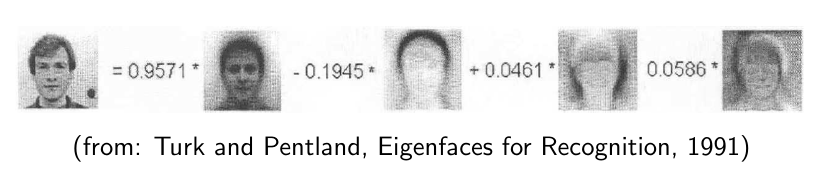
\includegraphics[scale=0.5]{\figDir/face_ex.PNG}
\end{figure}\\
The dimension of the original data points is the 
exact amount of pixels in the image. Perhaps the amount
of pixels is unmanageable. In this example, the faces were
are reconstructed using $k=4$ images. Thus, instead of 
considering each data point as a collection of pixels,
we reduced the dimension of the data by considering each data 
point as a combination of $4$ base images. We have reduced 
the dimension of the data to $4$. Of course, in order 
to re-construct the original images, the $4$ base images 
are required.
\end{exmp}

\section{Reducing data to a single value}
In order to see what PCA does exactly, we will first
consider what would happen if we reduced the $m$ dimensional
data to a single value. Hopefully, this value will contain 
the most information as possible. In essence we are looking 
at what would happen as $k = 1$. In order to reduce each data 
point to a single value, many approaches exist. Take for example
the approach where we simply take the euclidean norm of each point.
In this case, we capture some information but we lose a lot
of information. To see why consider $(0, 1)$ and $(1, 0)$.
They are perpendicular, yet $\norm{(0,1)} = \norm{(1,0)}$.
\\\\
There are better ways. We could for instance reduce the points
by projecting them onto a single line. This is actually the first
and only step in PCA. By iterating this exact step we obtain
the PCA decomposition. We start by projecting onto a single line.

\subsection{Projecting a single data point onto a fixed line}
Before we project onto it, we need to define exactly what 
is meant with a line in the $\Real^m$ space.
One way to define a line is as follows:

\begin{defn}
\begin{equation}
a + \Real b \equiv \{x \in \Real^m | 
\exists z \in \Real \text{ s.t. } x = a + zb\}
\end{equation}
Here, $a$ is sometimes referred to as the offset or intercept
and $b$ is sometimes referred to as the direction of the line.
\end{defn}
			
\begin{figure}[h!]
	\centering
	\begin{tikzpicture}[scale = 0.5]
	\draw[->] (-1,0) -- (5,0);
	\draw[->] (0,-1) -- (0,5);
	\draw[->, red, thick] (0,0) -- node[xshift = 1.5ex](lab){a}(1,2);
	\draw[->, blue, thick] (1,2) -- node[xshift = 1.5ex](lab){b}(2,1);
	\draw[blue, dashed] (-1,4) -- node[xshift = 1.5ex](lab){b}(4,-1);
	\end{tikzpicture}
	\label{fig:line}
	\caption{Visual of a line}
\end{figure}

Figure \ref{fig:line} gives an intuitive idea of 
what a line in $\Real^2$ looks like. Often we want the 
direction to have unit length. Mathematically this means: 
$\norm{b}_2 = 1$.
\\\\
Say we want to project a point $x$ onto a single line. There are
infinite ways to do this. However, if one wants to keep
as much of the information contained in the original 
point, we need to define an objective function.
Ideally, this objective function defines how distant the
projected point and the original point are. This concept 
should sound familiar. Just as in section \ref{sec:frobenius},
we defined the Frobenius norm as a metric to measure how
distance two matrices are. As the Frobenius norm is the 
natural extension of the $\mathcal{L}^2$ norm. Let's use 
the $\mathcal{L}^2$ norm to measure distance between
two points.
\\\\
We know that the projected point is somewhere on the line
we are projecting to. Let's call this point $a + bz$, we know
our line is fixed. This means $a$ and $b$ are fixed. Thus, the projected
point is completely defined by $z$. The squared euclidean
distance between the two points is then defined as:
\begin{equation}
\label{eq:eucl_proj}
\underset{z\in\Real}{\text{arg min}} \norm{a + bz - x}^2
\end{equation}

Figure \ref{fig:sq} shows an intuitive picture of 
the \textbf{non squared} euclidean distance. There are
\begin{figure}[h!]
	\centering
	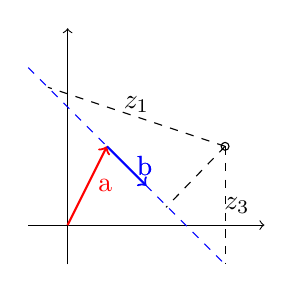
\begin{tikzpicture}[scale = 0.5]
	\draw[->] (-1,0) -- (5,0);
	\draw[->] (0,-1) -- (0,5);
					
	\draw (4,2) circle (0.1cm);
					
	\draw[->, red, thick] (0,0) -- node[xshift = 1.5ex](lab){a}(1,2);
	\draw[->, blue, thick] (1,2) -- node[xshift = 1.5ex](lab){b}(2,1);
	\draw[blue, dashed] (-1,4) -- node[xshift = 1.5ex](lab){b}(4,-1);
					
	\draw[dashed] (4,2) -- (2.5,0.45);
	\draw[dashed] (4,2) -- node[yshift = 1ex] {$z_1$} (-0.5,3.5);
	\draw[dashed] (4,2) -- node[xshift = 1ex] {$z_3$}(4,-1);
	\end{tikzpicture}
	\caption{Visual of distance to a line for varying $z$ values}
	\label{fig:sq}
\end{figure}\\

It is clear to see that using the squared euclidean distance 
that we reach the optimal point on the line by projecting the
original point orthagonally onto the line. 
Mathematically we can find this by deriving the squared
euclidean distance in equation \ref{eq:eucl_proj} for $z$.
\begin{equation}
\label{eq:sol_z}
\begin{split}
\der{z}\norm{a + bz - x}^2 &= 2(a +bz - x)^T b = 0 \\
&=(a-x)^T b + \underbrace{b^Tb }_{\norm{b}^2 = 1}z = 0\\
z &=-(a-x)^Tb
\end{split}
\end{equation}
This confirms our belief that the orthogonal projection 
does indeed minimize the distance between the original 
data point and the projected data point. We see this 
since we are projecting onto the $b$ direction.
\\\\
To understand 
exactly what's happening we can have a look at figure
\ref{fig:proj}. Here, the green arrow ($x-a$) is being 
projected onto $b$ to find the optimal $z$.
\begin{figure}[h!]
	\centering
	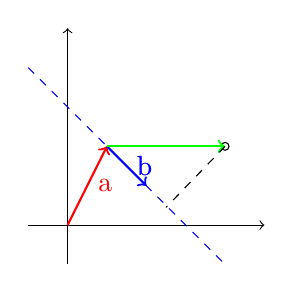
\begin{tikzpicture}[scale = 0.5]
	\coordinate[](origin) at (0,0) ;
	\coordinate[](a) at (1,2) ;
	\coordinate[](b) at (2,1) ;
	\coordinate[](x) at (4,2) ;
	
	\draw[->] (-1,0) -- (5,0);
	\draw[->] (0,-1) -- (0,5);
	
	\draw (x) circle (0.1cm);
	
	\draw[->, red, thick] (origin) -- node[xshift = 1.5ex](lab){a}(a);
	\draw[->, blue, thick] (a) -- node[xshift = 1.5ex](lab){b}(b);
	\draw[blue, dashed] (-1,4) -- node[xshift = 1.5ex](lab){b}(4,-1);
	
	\draw[thick, green, ->] (a)--(x);
	\draw[dashed] (4,2) -- (2.5,0.45);
	\end{tikzpicture}
	\caption{Visual of optimal $z$ value as a 
	projection of $(x-a)$ onto the direction.}
	\label{fig:proj}
\end{figure}
Now that we found the $z$ value that minimizes the 
loss (the projection onto the $b$ direction), let's look 
at what this means mathematically:
\begin{equation}
\label{eq:x_prime}
x' = a + (x-a)^Tbb
\end{equation} 
To better visualize this result, we can have a look at
figure \ref{fig:recon}.
\begin{figure}[h!]
	\centering
	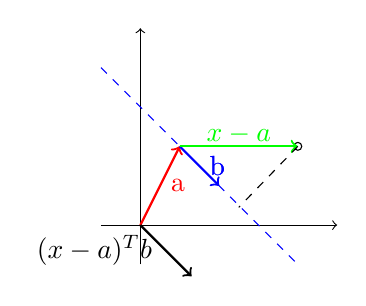
\begin{tikzpicture}[scale = 0.5]
	\coordinate[](origin) at (0,0) ;
	\coordinate[](a) at (1,2) ;
	\coordinate[](b) at (2,1) ;
	\coordinate[](x) at (4,2) ;
	
	\draw[->] (-1,0) -- (5,0);
	\draw[->] (0,-1) -- (0,5);
	
	\draw (x) circle (0.1cm);
	
	\draw[->, red, thick] (origin) -- node[xshift = 1.5ex](lab){a}(a);
	\draw[->, blue, thick] (a) -- node[xshift = 1.5ex](lab){b}(b);
	\draw[blue, dashed] (-1,4) -- node[xshift = 1.5ex](lab){b}(4,-1);
	
	\draw[thick, green, ->] (a)--node[yshift = 1ex]{$x-a$}(x);
	\draw[dashed] (4,2) -- (2.5,0.45);
	\draw[black, ->, thick] (origin) 
		--node[xshift = -6ex] {$(x-a)^Tb$} (1.3,-1.3);
	\end{tikzpicture}
	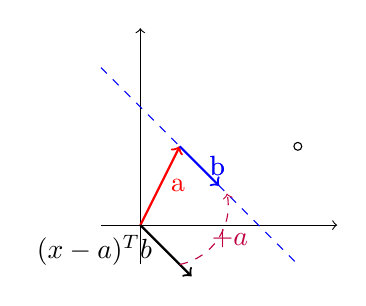
\begin{tikzpicture}[scale = 0.5]
	\coordinate[](origin) at (0,0) ;
	\coordinate[](a) at (1,2) ;
	\coordinate[](b) at (2,1) ;
	\coordinate[](x) at (4,2) ;
	
	\draw[->] (-1,0) -- (5,0);
	\draw[->] (0,-1) -- (0,5);
	
	\draw (x) circle (0.1cm);
	
	\draw[->, red, thick] (origin) -- node[xshift = 1.5ex](lab){a}(a);
	\draw[->, blue, thick] (a) -- node[xshift = 1.5ex](lab){b}(b);
	\draw[blue, dashed] (-1,4) -- node[xshift = 1.5ex](lab){b}(4,-1);
	\draw[black, ->, thick] (origin) 
			--node[xshift = -6ex] {$(x-a)^Tb$} (1.3,-1.3);
	
	\draw[dashed, ->, bend right = 45, purple]
		(1,-1)to node[xshift = 1ex]{$+a$}(2.2,0.8);
			
	\end{tikzpicture}
	\caption{Visual of optimal $z$ value 
			plugged back in to find the optimal point again.}
	\label{fig:recon}
\end{figure}
Mathematically, the story being told by equation \ref{eq:x_prime} is
quite logical. We can see 4 steps:
\begin{enumerate}
	\item Remove the intercept from $x$: $x-a$
	\item Project orthagonally onto $b$: $(x-a)^Tb$
	\item Multiply in the $b$ direction: $(x-a)^Tbb$
	\item Add back the intercept: $(x-a)^Tbb + a$
\end{enumerate}
So by minimizing the euclidean distance from a point
to a line we find the orthogonal projection. This will
be used extensively in the next few sections.

\subsection{Optimal line through multiple data points}
We've seen how to optimally project a single data 
point to a fixed line, minimizing euclidean distance.
We now look at what happens when we have more than a single
data point. Additionally, we don't consider the line $a + b\Real$
to be fixed. Instead, we turn the exercise upside down. We
want to answer the question: \textit{what would be the optimal
line through our data points, such that when we project all points
orthagonally, we keep as much information as possible?} In line
with the previous sections, we measure \textit{information} loss
using the euclidean distance.
\\\\
Mathematically, we wish to answer the following.
Consider $n$ data points $\{x_1,...,x_n\}$ where $x_i \in \Real^m$.
How do we find the optimal line considering the mean 
squared euclidean loss:
\begin{equation}
\label{eq:loss_ab}
L(a,b) = \frac{1}{n}\sum_{i=1}^{n}\norm{a + bz_i - x_i}
\end{equation}
Additionally we will consider $\norm{b} = 1$, $b$ is a unit 
length vector. This property will become important.
From previous the previous section, we already know that the optimal
$z_i$ for each individual data point in known to be 
$z_i = (x_i-a)^Tbb$. Due to the fact that one projection
of a data point does not interfere with another, we can simply
replace $z_i$ in equation \ref{eq:loss_ab}.
\\\\
Minimizing over $a$ and $b$ and using previous 
results of equation (\ref{eq:sol_z}) we find:

\begin{equation}
\label{eq:loss}
\begin{split}
\argmin_{a, b}\frac{1}{n}\sum_{i=1}^{n}\norm{a + bz_i - x_i}^2 &=
\argmin_{a, b}\frac{1}{n}\sum_{i=1}^{n}\norm{a + b(x_i - a)^Tb - x_i}^2
\\
&= \argmin_{a, b}\frac{1}{n}\sum_{i=1}^{n}
		\norm{bb^T(x_i - a) + (a - x_i)}^2 \\
&= \argmin_{a, b}\frac{1}{n}\sum_{i=1}^{n}
		\norm{bb^T(x_i - a) - (x_i - a)}^2 \\
&= \argmin_{a, b}\frac{1}{n}\sum_{i=1}^{n}
		\norm{(bb^T - \ID_{m})(x_i - a)}^2 \\
\end{split}
\end{equation}
Note that the $\norm{\cdot}$ operation is an even 
function so \ref{eq:loss} can be written equivalently
as (we can change the sign in the brackets 
$\norm{-a} = \norm{a}$):
\begin{equation}
\argmin_{a, b}\frac{1}{n}\sum_{i=1}^{n}\norm{(\ID - bb^T)(x_i - a)}^2 \\
\end{equation}
Now what exactly does the $(\ID_m - bb^T)$ transformation mean?
Transforming a vector $v$ out we obtain:
\begin{equation}
(\ID_m - bb^T)v = v - b(b^Tv)
\end{equation}
Reminding ourselves that $b$ is a unit vector, we can see it
is exactly the vector we obtain when taking the difference
between an original vector $v$ and the projection of the vector
$b(b^Tv)$. Unsurprisingly of course, as that is exactly what we 
started with.
\\\\
A nice thing about $(\ID - bb^T)$ is that it is idempotent.
We can show that this is clearly the case:
\begin{equation}
\label{eq:idempot}
\begin{split}
	(\ID -bb^T)(\ID - bb^t) &= \ID\ID - 2bb^T 
			+ b\underbrace{b^Tb}_{b^Tb = \norm{b}}b^T\\
&= \ID - bb^T\\
\end{split}
\end{equation}\\

\subsection{Optimal value for $a$}
Now let's get back to finding the optimal line for given data. 
The first order optimality condition states that the gradient
with respect to $a$ and $b$ should vanish when optimal.
Taking the gradient with respect to $a$ 
of equation \ref{eq:loss} we find the following:
\begin{equation}
\label{eq:grad_Lin_loss_1}
\begin{split}
\nabla_a L(a,b) &=  \frac{1}{n}\sum_{i=1}^{n}
	\nabla_a\norm{(\ID - bb^T)(x_i - a)}^2 \\
&= \frac{-2}{n}\sum_{i=1}^{n}
	(\ID - bb^T)^T(\ID - bb^T)(x_i - a) \\
&= \frac{-2}{n}(\ID - bb^T)^T
	(\ID - bb^T)\sum_{i=1}^{n}(x_i - a) \\
\end{split}
\end{equation}
In the second line we used the fact that $\nabla_x \norm{Ax}^2 = 2AxA^T$,
which was proven in the definitions section.
We now know that since $(\ID - bb^T)$ is clearly symmetric 
($A^T = A$) and we know that the matrix is idempotent from 
(\ref{eq:idempot}), thus we can write 
(\ref{eq:grad_Lin_loss_1}) follows:
\begin{equation}
\label{eq:grad_Lin_loss_2}
\begin{split}					
	\nabla_a L(a,b) = (\ID - bb^T)\sum_{i=1}^{n}(x_i - a) &= 0\\
	(\ID - bb^T)\sum_{i=1}^{n}(x_i) &= (\ID - bb^T)\sum_{i=1}^{n}(a)\\
	(\ID - bb^T)\frac{1}{n}\sum_{i=1}^{n}(x_i) &= (\ID - bb^T)a\\
\end{split}
\end{equation}
From (\ref{eq:grad_Lin_loss_2}) we can see that the 
optimality condition is met when $a = \frac{1}{n}\sum_{i=1}^{n}x_i$.
This means that the optimal line will always pass through 
the average of all the data points. Figure \ref{fig:avg} 
shows this visually:\\
\begin{figure}[h!]
	\centering				
	\begin{tikzpicture}[scale=0.8]
	\coordinate[](origin) at (0,0) ;
	\coordinate[](x1) at (4,3) ;
	\coordinate[](x2) at (1,2.5) ;
	\coordinate[](x3) at (2,0.5);
	\coordinate[blue](av) at (2.3333333, 2);
	
	\draw (x1) circle (0.1);
	\draw (x2) circle (0.1);
	\draw (x3) circle (0.1);
	\draw[blue, thick, fill = blue] (av) 
			circle (0.05) node[xshift = 2ex]{$\bar{x}$};
	
	\draw[dashed, red] (origin) -- (4.666,4) node[]{$l_1$};
	\draw[dashed, red] (-1,2) -- (5, 2) node[]{$l_2$};
	\draw[dashed, red] (0,4.3333) -- (5,-0.66666) node[]{$l_3$};
	
	\draw[dotted] (av)--(x1) node[xshift = 2ex]{$x_1$};
	\draw[dotted] (av)--(x2) node[xshift = -2ex]{$x_2$};
	\draw[dotted] (av)--(x3) node[xshift = -2ex]{$x_3$};
	
	\draw[->] (-1,0) -- (5,0);
	\draw[->] (0,-1) -- (0,5);
	\end{tikzpicture}
	\caption{Visualisation of lines going 
		through average of data points $x_i$.}
\label{fig:avg}
\end{figure}\\
Figure \ref{fig:avg} shows us visually something quite
interesting, since we know that the optimal line passes 
through the average $\bar{x}$ we could try to make the 
origin itself the average. We could achieve this by 
subtracting the average from every data point as shown 
in figure \ref{fig:subavg}. This step is very often done
as a pre-processing step. It makes derivations easier 
analytically. When "data is centered", this simply means 
that the empirical mean $\frac{1}{n}\sum_{i=1}^{n}x_i$ 
has already been subtracted and that the new mean is the origin.
			
\begin{figure}[h!]
	\centering				
	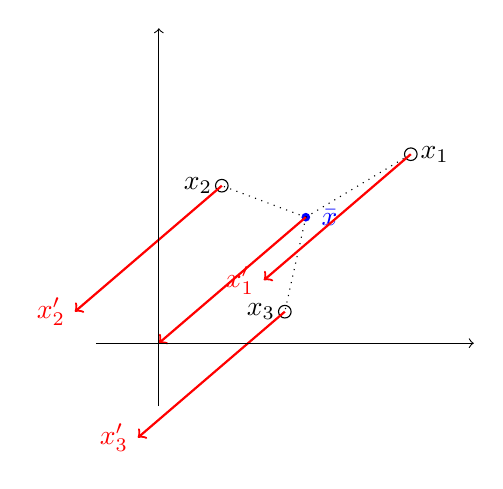
\begin{tikzpicture}[scale=0.8]
	\coordinate[](origin) at (0,0) ;
	\coordinate[](x1) at (4,3) ;
	\coordinate[](x2) at (1,2.5) ;
	\coordinate[](x3) at (2,0.5);
	\coordinate[blue](av) at (2.3333333, 2);
	
	\draw (x1) circle (0.1);
	\draw (x2) circle (0.1);
	\draw (x3) circle (0.1);
	\draw[blue, thick, fill = blue] (av) 
			circle (0.05) node[xshift = 2ex]{$\bar{x}$};
	
	\draw[dotted] (av)--(x1) node[xshift = 2ex]{$x_1$};
	\draw[dotted] (av)--(x2) node[xshift = -2ex]{$x_2$};
	\draw[dotted] (av)--(x3) node[xshift = -2ex]{$x_3$};
	
	\draw[thick, red, ->] (av) -- (origin);
	\draw[thick, red, ->] (x1) -- ++(-2.33333,-2)node[xshift = -2ex]{$x_1'$};
	\draw[thick, red, ->] (x2) -- ++(-2.33333,-2)node[xshift = -2ex]{$x_2'$};
	\draw[thick, red, ->] (x3) -- ++(-2.33333,-2)node[xshift = -2ex]{$x_3'$};
					
	\draw[->] (-1,0) -- (5,0);
	\draw[->] (0,-1) -- (0,5);
	\end{tikzpicture}
	\caption{Visualisation of substracting mean of points from $x_i$.}
	\label{fig:subavg}
\end{figure}

\subsection{Optimal value for $b$ as principal eigenvectors}
As figure \ref{fig:avg} suggests, this of course leaves 
the question of \textit{How do we choose the direction of the optimal line?}
From now, we will assume the data is centered, this means that
$a$ in $a+bz$ is assumed to be $0$. If we then look at the 
euclidean loss function as in (\ref{eq:loss}), 
where $a=0$:
\begin{equation}
	\begin{split}
	L(b) &= \frac{1}{n}
		\sum_{i=1}^{n}\norm{x_i^Tbb - x_i}^2 \\
	L(b) &= \frac{1}{n}\Bigg(
		\sum_{i=1}^{n}\norm{x_i^Tbb}^2 +
		\sum_{i=1}^{n} \norm{x_i}^2 - 
		2\sum_{i=1}^{n} (x_i^Tbb)^Tx_i \Bigg)\\
	\end{split}		
	\label{eq:loss_decomposed}		
\end{equation}
Rewriting $\norm{x_i^Tbb}^2$ we find:
\begin{equation}
\norm{x_i^Tbb}^2 = (x_i^Tbb)^Tx_i^Tbb = 
	(x_i^Tb)\underbrace{b^Tb}_{=1}b^Tx_i = \norm{x_i^Tb}^2
\end{equation}
Further observing that $(x_i^Tbb)^Tx_i = (x_i^Tb)b^Tx_i = \norm{x_i^Tb}^2$,
leaves us with the re-written loss function from equation
\ref{eq:loss_decomposed}:
\begin{equation}
\begin{split}
L(b) = \frac{1}{n}\Bigg(
	-\sum_{i=1}^{n}\norm{x_i^Tbb}^2 +
	\sum_{i=1}^{n} \norm{x_i}^2\Bigg)\\
\end{split}	
\end{equation}
Aditionally since $\norm{x_i}^2$ is constant it can be 
left out from (\ref{eq:loss_decomposed}), when minimizing
for $b$. This results in:
\begin{equation}
\begin{split}
	L(b) = \frac{-1}{n}\sum_{i=1}^{n} \norm{x_i^Tb}^2 \\
\end{split}			
\end{equation}
Now we have simplified what we want to minimize, let's 
see what exactly is going on. Let's take the mathematical
route for now:
\begin{equation}
\label{eq:sample_var}
\begin{split}
	b&\in\argmin_{b, \norm{b} = 1}
		\frac{-1}{n}\sum_{i=1}^{n} \norm{x_i^Tb}^2 \\
	b&\in\argmax_{b, \norm{b} = 1}
		\frac{1}{n}\sum_{i=1}^{n} (x_i^Tb)^T(x_i^Tb) \\
	b&\in\argmax_{b, \norm{b} = 1} 
		b^T\Big(\frac{1}{n}\sum_{i=1}^{n} x_ix_i^T\Big)b \\					
	b&\in\argmax_{b, \norm{b} = 1}
		 b^T \Sigma b \\
\end{split}			
\end{equation}
In (\ref{eq:sample_var}) we find that $\Sigma = 
\frac{1}{n}\sum_{i=1}^{n} x_ix_i^T$ is simply the sample 
covariance matrix\footnote{Note that we already assumed that
the data is centered, thus $\Sigma$ can indeed be 
considered the sample covariance matrix.}!
We can now try to minimize this constrained objective.
Note that we assumed that $\norm{b}=1$, 
we can use a Lagrange multiplier to in order to turn 
the constrained objective into the unconstrained objective:

\begin{equation}
\label{eq:lagrange}
\mathcal{L}(b,\lambda) = b^T\Sigma b + \lambda\norm{b}^2	
\end{equation}
Finding the extremal value of (\ref{eq:lagrange}) we
derive for $b$ and equal the gradient to 0, as usual:
\begin{equation}
\label{eq:optimality_cond_b}
\begin{split}
\nabla_b\mathcal{L}(b,\lambda) = (2\Sigma b - 2\lambda b) &= 0\\
\Sigma b &= \lambda b\\
\end{split}			
\end{equation}
So we have derived that the optimal $b$ is actually 
an eigenvector of the $\Sigma$ matrix. The Lagrange 
multiplier $\lambda$ is the corresponding eigenvalue.
The question still remains, \textit{which eigenvector
will maximize $b^T\Sigma b$?}
\\\\
We can maximize $b^TXb$ when $b$ is the eigenvector
which has the highest eigenvalue. To see exactly why 
this is the case we look again at the Lagrangian in 
(\ref{eq:lagrange}) and plug in the optimality 
condition from equation \ref{eq:optimality_cond_b}:
\begin{equation}
\begin{split}
\mathcal{L}(b,\lambda) 
&= 
	\lambda \underbrace{b^Tb}_{=1} + 
	\lambda\norm{b}^2 \\
&= 
	2\lambda \\
\end{split}
\end{equation}
Since we are maximizing, $\lambda$ should be as 
large as possible. The eigenvector that has the 
highest eigenvalue is called the \textit{principal} 
eigenvector or $\Sigma$.

\subsection{Optimal value of $b$ as projected data variance.}
We saw that the optimal direction is actually just 
the principal eigenvector of the covariance matrix $\Sigma$.
Let's look at the loss function again from a different
perspective. Let's look again at what it means to maximize 
$b^T\Sigma b$. From (\ref{eq:sample_var}) we know that:

\begin{equation}
b^T\Sigma b 
= \frac{1}{n}\sum_{i=1}^{n}\norm{x_i^Tb}^2 
= \frac{1}{n}\sum_{i=1}^{n}z_i^2 
= \frac{1}{n}\sum_{i=1}^{n}(z_i - 0)^2
\end{equation}

Note that this is simply the empirical (biased) variance of
the projected data points, since the projected mean is 
exactly the projection of the origin (centered data) onto
the line going through the origin. Thus the projected mean
is also $0$. We can thus interpret this as:
\begin{equation}
	b^T\Sigma b = Var[z]
\end{equation}
So we can either interpret the objective in two ways.
One as finding the principal eigenvector of the sample 
covariance matrix or as the maximization of the projected
data. Figure \ref{fig:projected_variance} below shows this visually:
\begin{figure}[h!]
	\centering
	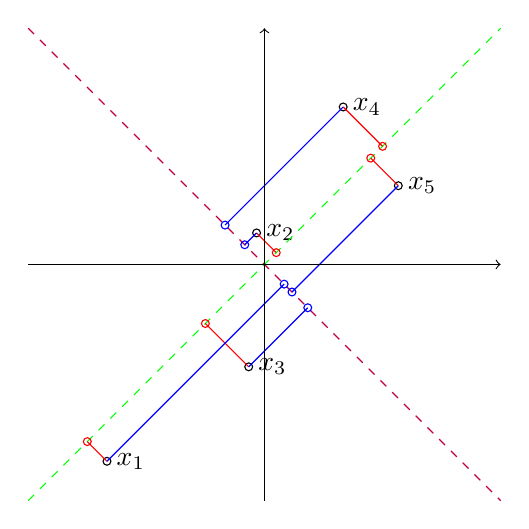
\begin{tikzpicture}
	\coordinate[](origin) at (0,0) ;
	\coordinate[](x1) at (-2,-2.5) ;
	\coordinate[](x2) at (-0.1,0.4) ;
	\coordinate[](x3) at (-0.2,-1.3);
	\coordinate[](x4) at (1,2);
	\coordinate[](x5) at (1.7, 1);
	
	\draw[](x1)circle (0.05) node[xshift=2ex]{$x_1$};
	\draw[](x2)circle (0.05) node[xshift=2ex]{$x_2$};
	\draw[](x3)circle (0.05) node[xshift=2ex]{$x_3$};
	\draw[](x4)circle (0.05) node[xshift=2ex]{$x_4$};
	\draw[](x5)circle (0.05) node[xshift=2ex]{$x_5$};
	
	\draw[dashed, green](-3,-3)--(3,3);
	\draw[red](x1)--(-2.25,-2.25) circle (0.05);
	\draw[red](x2)--(0.15,0.15) circle (0.05);
	\draw[red](x3)--(-0.75,-0.75) circle (0.05);
	\draw[red](x4)--(1.5,1.5) circle (0.05);
	\draw[red](x5)--(1.35,1.35) circle (0.05);
	
	\draw[dashed, purple](-3,3)--(3,-3);
	\draw[blue,thin](x1)--(.25,-.25) circle (0.05);
	\draw[blue,thin](x2)--(-0.25,0.25) circle (0.05);
	\draw[blue,thin](x3)--(0.55,-0.55) circle (0.05);
	\draw[blue,thin](x4)--(-0.5,0.5) circle (0.05);
	\draw[blue,thin](x5)--(0.35, -0.35) circle (0.05);
	
	\draw[->] (-3,0) -- (3,0);
	\draw[->] (0,-3) -- (0,3);
	\end{tikzpicture}
	\caption{Visual of projected variance maximization.}
	\label{fig:projected_variance}
\end{figure}
Clearly the purple line has lower projected variance 
than the green line. Intuitively the worst case line 
would project all points onto the same point, losing 
all information (variance). The best case would 
maximize the the variance. Variance of the projections
can then be seen as how much information is retained 
when projecting.

\section{Principal Component Analysis(PCA)}
We've seen the case of a single line, now we could 
ask ourselves, \textit{Could we perform another 
projection?}. Let's take a look at the so called 
\textit{residual}, which is the original data point
minus the projected data point. In essence what the
residuals mean is the original signal (data point)
when removing all signal in the principal direction.
\begin{equation}
\label{eq:residual_definition}
\begin{split}
	 r_i := x_i - (a + bz_i) &= x_i - (x_i)^Tbb\\
	 &=(\ID - bb^T)x_i
\end{split}
\end{equation}
The above result was derived using $x_i^Tbb = 
bx_i^Tb=bb^Tx_i$. Figure \ref{fig:residual} shows
what the residuals looks like, however since there
are only $2$ dimensions it's somewhat less clear.
\begin{figure}[h!]
	\centering
	\begin{tikzpicture}
	\coordinate[](origin) at (0,0) ;
	\coordinate[](x1) at (-2,-2.5) ;
	\coordinate[](x2) at (-0.1,0.4) ;
	\coordinate[](x3) at (-0.2,-1.3);
	\coordinate[](x4) at (1,2);
	\coordinate[](x5) at (1.7, 1);
	
	\draw[](x1)circle (0.05) node[xshift=2ex]{$x_1$};
	\draw[](x2)circle (0.05) node[xshift=2ex]{$x_2$};
	\draw[](x3)circle (0.05) node[xshift=2ex]{$x_3$};
	\draw[](x4)circle (0.05) node[xshift=2ex]{$x_4$};
	\draw[](x5)circle (0.05) node[xshift=2ex]{$x_5$};
	
	\draw[dashed, green](-3,-3)--(3,3);
	\draw[->, red](x1)->(-2.25,-2.25) circle (0.05);
	\draw[->, red](x2)->(0.15,0.15) circle (0.05);
	\draw[->, red](x3)->(-0.75,-0.75) circle (0.05);
	\draw[->, red](x4)->(1.5,1.5) circle (0.05);
	\draw[->, red](x5)->(1.35,1.35) circle (0.05);
	
	\draw[->](origin) -- (0.25,-0.25);
	\draw[->](origin) -- (-0.25,0.25);
	\draw[->](origin) -- (0.55,-0.55);
	\draw[->](origin) -- (-0.5, 0.5);
	\draw[->](origin) -- (0.35,-0.35);
	
	\draw[->] (-3,0) -- (3,0);
	\draw[->] (0,-3) -- (0,3);
	\end{tikzpicture}
	\caption{Visualisation of residuals.}
	\label{fig:residual}
\end{figure}

\subsection{PCA as an iterative process}
What if we project the residuals to an optimal line. 
We simply treat the residuals as our new data. Note that
the analysis to do this is exactly the same case as in 
previous sections. We also need the fact that the mean
of the residuals is again centered since:
\begin{equation}
\frac{1}{n}\sum_{i=1}^{n}r_i 
	= (\ID - bb^T)\frac{1}{n}\sum_{i=1}^{n}x_i = 0
\end{equation}
This means that the analysis can be done exactly the 
same. Like in previous section, minimizing $\sum_{i-1}^{n}
\norm{r_i^Tbb - r_i}^2$ for b will result in having 
to maximize $b^T(\frac{1}{n}\sum_{i=1}^{n}r_ir_i^T)b 
= b^T\Sigma_rb$ for b. 
\\\\
We could simply find the principal eigenvector of 
$\Sigma_r $ and do this iteratively, but maybe we could 
exploit a relationship to make it simpler? So what exactly is the 
relationship between $\Sigma_r$ and $\Sigma$? We analyse 
this as follows using (\ref{eq:residual_definition}), the
fact that $(\ID - bb^T)$ is idempotent as shown in equation 
(\ref{eq:idempot}) and that $\Sigma$ is symmetric:
\begin{equation}
\label{eq:residuals_loss}
\begin{split}
\frac{1}{n}\sum_{i=1}^{n}r_ir_i^T 
	&= \frac{1}{n}\sum_{i=1}^{n}(\ID - bb^T)x_i((\ID - bb^T)x_i)^T\\
	&= \frac{1}{n}\sum_{i=1}^{n}(\ID - bb^T)x_ix_i^T(\ID - bb^T)^T\\
	&= (\ID - bb^T)\Sigma(\ID - bb^T)^T \\
	&= (\ID - bb^T)(\ID - bb^T)\Sigma^T \\	
	&= \Sigma - b\Sigma b^T\\
	&= \Sigma - \lambda bb^T			
\end{split}
\end{equation}
Note that in line 4 in equation \ref{eq:residuals_loss}
we used the fact that $(\ID - bb^T)$ and $\Sigma$ are symmetric, 
which implies $\Sigma (\ID - bb^T) = (\ID - bb^T) \Sigma$.
We can already notice something important, $b$ 
(the eigenvector of $\Sigma$) is now also an eigenvector
of $(\Sigma - \lambda bb^T)$:
\begin{equation}
(\Sigma - \lambda bb^T)b = \Sigma b - \lambda b = 0\\
\end{equation}

The reverse is obviously true an eigenvector of 
$(\Sigma - \lambda bb^T)$ is also an eigenvector of
$\Sigma$, it follows from the previous. This $v$ is 
the principal eigenvector of $(\Sigma - \lambda bb^T)$ 
(by construction) and the second principle eigenvector 
of $\Sigma$, by iterating $m$ times we find $m$ pairwise 
orthogonal eigenvectors. Figure \ref{fig:residual} shows 
visually that using the residuals to find an optimal 
projection will find maximum projected variance when 
the line is orthogonal to the green line. Another way to 
see why they are orthogonal is by noting that $\Sigma$ is 
positive semi-definite ($\lambda_i > 0$) because it's 
symmetric so the eigenvectors are orthogonal\footnote{say 
$x$ and $y$ are eigenvectors with $\lambda_1$ and 
$\lambda_2$ as eigenvalues of $A$ then $\lambda_1 <x,y> 
= <Ax,y> = <x,A^Ty> = <x,Ay>=<x,y>\lambda_2$ since $\lambda_1
\neq \lambda_2$ then $<x,y>=0$.}.

\subsection{PCA as a diagonalization problem}
Recall that $\Sigma$ is symmetric so it may be diagonalized into orthogonal matrices:
\begin{equation}
\Sigma = U\Lambda U^T
\end{equation}
Where $U=(u_1, u_2, \dots, u_m)$ and $\Lambda = diag(\lambda_1, \dots, \lambda_m)$ note that the eigenvectors are orthogonal so that:
\begin{equation}
	U^Tu_i = \begin{bmatrix}
	u_1^T\\
	\vdots\\
	u_m^T
	\end{bmatrix}u_i = \begin{bmatrix}
	u_1^Tu_i\\
	\vdots\\
	u_m^Tu_i
	\end{bmatrix} = \begin{bmatrix}
	0\\
	\vdots\\
	u_i^Tu_i = 1\\
	\vdots\\
	0\\
	\end{bmatrix}=e_i
\end{equation}
Using this we can clearly see that:
\begin{equation}
\begin{split}
	U\Lambda U^T & =\begin{bmatrix}
	u_1 & \dots & u_m\\
	\end{bmatrix}
	\begin{bmatrix}
	\lambda_1 &\dots & 0\\
	\vdots&\cdots&\vdots\\
	0& \dots& \lambda_m\\
	\end{bmatrix}
	\begin{bmatrix}
	u_1 \\ \vdots \\ u_m\\
	\end{bmatrix}		\\
	&=\begin{bmatrix}
	\lambda_1u_1 & \dots & \lambda_mu_m\\
	\end{bmatrix}\begin{bmatrix}
	u_1 \\ \vdots \\ u_m\\
	\end{bmatrix}\\
	&= \Sigma \underbrace{UU^T}_{\ID} = \Sigma
\end{split}
\end{equation}
In order to then reduce the dimension of the data we
would simply project our data onto the $k$ principal
components:
\begin{equation}
Z = U_k^T X
\end{equation}

\subsection{Colclusion: PCA}
Let's recap what we did to find out what PCA is.
\\\\
First we investigated that the orthogonal projection
is the optimal projection of a data point onto a line
considering the euclidean distance as loss measure.
\\\\
Second we looked at finding the optimal line onto which
we could project our data such that we keep as much
information as possible. As it turned out, the optimal
intercept $a$ is exactly the mean of all the points.
The optimal $b$ turned out to be the principal component
of the sample covariance matrix. Alternatively, the $b$
direction is exactly the direction which maximizes the 
projected variance of the points.
\\\\
Thirdly we looked at iteratively projecting the residuals
onto the optimal line. This is exactly what PCA does.
Another way to look at it was as a diagonalization 
problem of $\Sigma = U\Lambda U^T$.
\\\\
Now where is the \textit{reduction} of the data exactly? 
Well every point can be projected to $d$ principle 
eigenvectors of $\Sigma$ to give us $U^T x_i = 
(u_1^Tx_i \dots u_d^Tx_i) = (z_1 \dots z_d)$ this gives 
us a reduction to the optimal weights for a linear combination 
of the lower dimensional basis (the $d$ principal eigenvectors). 
To re-construct the data point we take a linear combination of 
the $d$ principal eigenvectors. This can be done as 
$(z_1 \dots z_d)U$. Of course when you pick $d$ to be the 
dimension of the data then there is no reduction but an 
exact decomposition of the data matrix $X$. So basically:

\begin{itemize}
 	\item Reduction: 
 	\begin{equation}
 	Z 
 	= U^T X
 	= 
 	\begin{pmatrix}
 	\horzbar & u_1 & \horzbar\\
 	 & \vdots & \\
 	\horzbar & u_d & \horzbar\\
 	\end{pmatrix}
 	\begin{pmatrix}
 	\vertbar & & \vertbar \\
 	x_1 & \dots & x_n\\
 	\vertbar & & \vertbar \\
 	\end{pmatrix} 
 	= 
 	\begin{pmatrix}
 	z_{1,1} & \dots& z_{n,1}\\
 	\vdots& \ddots & \vdots\\
 	z_{1,d} & \dots & z_{n,d}\\
 	\end{pmatrix}
 	\end{equation}
we can clearly see that we reduced the data from $\Real^m$ 
to $\Real^d$. Only if $d < m$ is there really a reduction 
and is there truly an approximation when reconstructing!
 	\item Re-construction:
 	\begin{equation}
 	\hat{X} = UZ = \begin{bmatrix} 
 	\sum_{i=1}^{d}z_{1,i}u_i & \dots & \sum_{i=1}^{d}z_{n,i}u_i \\
 	\end{bmatrix}
 	\end{equation}
Here I wrote it out explicitly so it's easy to see that 
the reduction is just keeping track of weights for the 
linear combination of the $d$ principal eigenvectors.
\end{itemize}
		 
\section{Practical PCA: Finding pricipal eigenvector}
We've seen a derivation of PCA, one perspective of PCA 
is iteratively finding principal eigenvectors or certain 
symmetric matrices (empirical biased covariance matrix of 
the data or residuals). However we skipped the part where 
we actually find the principal eigenvector. One practical 
way of finding the principal eigenvector is the 
\textit{power method}.

\subsection{Power method: practical principal eigenvector}
Assume a symmetric matrix $\Sigma$ and we wish 
to find $u_1$, the principal eigenvector of $\Sigma$. 
The algorithm goes as follows:
\begin{enumerate}
	\item Initialize $v_0$ a random vector. For simplicity 
	we assume that $\langle u_1,v_0\rangle \neq 0$ and that 
	the principal eigenvalue is unique i.e. $|\lambda_1| > |\lambda_j|$.
	
	\item Iteratively apply the following operation:
	\begin{equation}
	v_{t+1} = \frac{\Sigma v_t}{\norm{\Sigma v_t}}
	\end{equation}
	 
	\item It holds that:
	\begin{equation}
	\lim_{t\rightarrow\infty} v_t = u_1
	\end{equation}
	 
	\item To find the corresponding eignenvalue:
	\begin{equation}
	\lambda_1 
		= \lim_{t\rightarrow\infty} \frac{\norm{\Sigma v_t}}{\norm{v_t}} 
		= \frac{\norm{\Sigma u_1}}{\norm{u_1}} 
		= \frac{\norm{\lambda_1u_1}}{\norm{u_1}} 
	\end{equation}
\end{enumerate}

\noindent
Why does this algorithm work? We assume $\Sigma$ (as in last
section) is p.s.d. and symmetric (true for $XX^T$). In this 
case the eigenvectors are all orthogonal to each other so they 
form a basis for $\Real^m$, this means any $v_0 \in \Real^m$ 
can be written as a linear combination of eigenvectors:

\begin{equation}
\label{eq:eigenbasis}
v_0 = \sum_{i=1}^{m} a_i u_i
\end{equation}

\noindent 
how does $v_t$ evolve considering this?

\begin{equation}
\label{eq:evolve_power}
v_{t} 
	= \frac{\Sigma^t v_0}{\norm{\Sigma^t v_0}} 
	= \frac{\sum_{i=1}^{m}a_i\Sigma^t u_i}{\norm{\Sigma^t v_0}}
\end{equation}

\noindent 
Note equation (\ref{eq:evolve_power}) was obtained by 
recursively finding $v_i$ and using (\ref{eq:eigenbasis}). 
Since $u_i$ are eigenvectors by assumption we can re-write 
it as follows by pulling out the highest eigenvalue:

\begin{equation}
\frac{a_1\lambda_1^tu_1 
+ \sum_{i=2}^{m}\frac{a_i}{a_1}
(\frac{\lambda_i}{\lambda_1})^t u_i}
{\norm{\Sigma^t v_0}}
\end{equation}

\noindent
To understand the limit as $t\rightarrow\infty$ we 
see for the numerator:
	
\begin{equation}
\lim_{t\rightarrow\infty}a_1\lambda_1^tu_1 
	+ \sum_{i=2}^{m}\frac{a_i}{a_1}
	(\underbrace{\frac{\lambda_i}{\lambda_1}}_{=0})^t u_i 
	= a_1\lambda_1^tu_1
\end{equation}
The denomenator can be interpreted in the same way 
(using $\norm{u_1} = 1$), cancelling the $a_1\lambda_1^t$ 
resulting in power iteration method converging to $u_1$.
	
\section{Practical PCA: choosing amount of eigenvectors}
How many eigenvectors should we \textit{select} or \textit{keep}
and how should we select which ones to keep and not keep. 
Intuitively from previous section which looked at PCA as a 
variance maximisation of the projected data, we should keep 
the $k$ eigenvectors which have the highest eigenvalues. It 
represents how much information is contained within the 
eigenvector for specific data.
\\\\
This leaves the question, how many of the top eivenvectors 
should we keep? This has to be decided in a more empirical way, 
for example one could gather all eigenvalues and sort them and 
plot their value against index as follows:
	
\begin{figure}[h!]
\centering
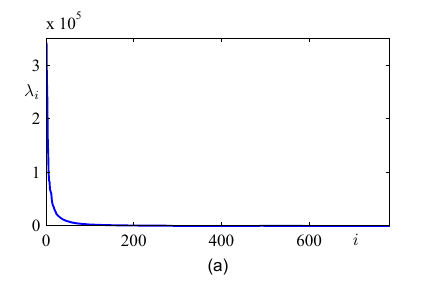
\includegraphics[scale = 0.7]{\figDir/eigenspectrum.PNG}
\label{fig:eigenspectrum}
\caption{Sorted eigenvalues plotted against index}
\end{figure}

\noindent
In this case it seems like taking the top 50 eigenvectors 
to represent a reduced dataset would be a good approximation. 
An engineering rule would be to cut off at \textit{the knee} 
where the eigenspectrum starts to plateau rapidly.
